 \documentclass[oneside,a4paper,12pt]{book}
%\pagestyle{headings}
\frontmatter

%=============================================================================

\usepackage{amsthm}
\usepackage{xspace}
\usepackage{float}
\usepackage{ifthen}
\usepackage{amsbsy}
\usepackage{amssymb}
\usepackage{balance}
\usepackage{booktabs}
\usepackage{graphicx}
\usepackage{rotating}
\usepackage{multirow}
\usepackage{needspace}
\usepackage{microtype}
\usepackage{bold-extra}
\usepackage{geometry}
\usepackage{varioref}
\usepackage{xcolor}
\usepackage{textcomp}
\usepackage{listings}
\usepackage[normalem]{ulem} %emphasize still italic
\usepackage{ucs}

% \usepackage[utf8]{inputenc}
% \usepackage[htt]{hyphenat}
\usepackage{times}
\usepackage{url}
\usepackage{alltt}
\usepackage{amsmath}
\usepackage{xfrac}
\usepackage{subfigure}
\usepackage{appendix}
\usepackage{stmaryrd}   % for the \shortuparrow
\usepackage[utopia]{quotchap}

\usepackage{setspace}
\usepackage[numbers, sort&compress]{natbib}
\usepackage{mdwlist}        % support for better spaced lists
% allows for temporary adjustment of side margins
\usepackage{chngpage}
\usepackage[normalem]{ulem} 

% lina entered
\usepackage{indentfirst}
\usepackage[parfill]{parskip}
\usepackage[bottom]{footmisc}

\usepackage[T1]{fontenc}
\usepackage{caption}
\usepackage{booktabs}
\usepackage{siunitx}


\setlength{\parindent}{1.5em}

% constants

\newcounter{qcounter}

% commands
\newcommand{\n}{$\cdot$}
\newcommand{\y}{\checkmark}
\newcommand{\subscript}[1]{$_{\textrm{\footnotesize{#1}}}$}
\newcommand{\superscript}[1]{$^{\textrm{\footnotesize{#1}}}$}
\newcommand{\vertical}[1]{\raisebox{-4em}{\begin{sideways}{#1}\end{sideways}}}
\newcommand\tab[1][1cm]{\hspace*{#1}}

\usepackage{boxedminipage}

\newboolean{showedits}
\setboolean{showedits}{true} % toggle to show or hide edits
\ifthenelse{\boolean{showedits}}
{
       \newcommand{\ugh}[1]{\textcolor{red}{\uwave{#1}}} % please rephrase
       \newcommand{\ins}[1]{\textcolor{blue}{\uline{#1}}} % please insert
       \newcommand{\del}[1]{\textcolor{red}{\sout{#1}}} % please delete
       \newcommand{\chg}[2]{\textcolor{red}{\sout{#1}}{\ra}\textcolor{blue}{\uline{#2}}} % please change
}{
       \newcommand{\ugh}[1]{#1} % please rephrase
       \newcommand{\ins}[1]{#1} % please insert
       \newcommand{\del}[1]{} % please delete
       \newcommand{\chg}[2]{#2}
}


% ============================================================================
% Put edit comments in a really ugly standout display

\usepackage{xcolor}
\usepackage[normalem]{ulem}
\newcommand{\ra}{$\rightarrow$}
\usepackage{amssymb}

% comments \nb{label}{color}{text}
\newboolean{showcomments}
\setboolean{showcomments}{true}
%\setboolean{showcomments}{false}
\ifthenelse{\boolean{showcomments}}
{\newcommand{\nb}[3]{
  {\colorbox{#2}{\bfseries\sffamily\scriptsize\textcolor{white}{#1}}}
  {\textcolor{#2}{\sf\small$\blacktriangleright$\textit{#3}$\blacktriangleleft$}}}
    \newcommand{\version}{\emph{\scriptsize$-$Id$-$}}
%	 \newcommand{\ugh}[1]{\textcolor{red}{\uwave{#1}}} % please rephrase
%	 \newcommand{\ins}[1]{\textcolor{blue}{\uline{#1}}} % please insert
%	 \newcommand{\del}[1]{\textcolor{red}{\sout{#1}}} % please delete
%	 \newcommand{\chg}[2]{\textcolor{red}{\sout{#1}}{\ra}\textcolor{blue}{\uline{#2}}} % please change
	 \newcommand{\chk}[1]{\textcolor{ForestGreen}{#1}} % changed, please check
	}
{\newcommand{\nb}[3]{}
  \newcommand{\version}{}
  \newcommand{\chk}[1]{} % changed, please check
  }
\newcommand\nm[1]{\nb{NM}{violet}{#1}} % add more author macros here
\newcommand\lt[1]{\nb{LT}{orange}{#1}}


% ============================================================================
% Make quotes be italic
\renewenvironment{quote}
    {\list{}{\rightmargin\leftmargin}%
     \item\relax\begin{it}}
    {\end{it}\endlist}

\newcommand{\ttimes}{\ensuremath{\times}}

%=============================================================================

\newcommand{\needlines}[1]{\Needspace{#1\baselineskip}}

% source code
\usepackage{xcolor}
\usepackage{textcomp}
\usepackage{listings}
\definecolor{javared}{rgb}{0.6,0,0} % for strings
\definecolor{javagreen}{rgb}{0.25,0.5,0.35} % comments
\definecolor{javapurple}{rgb}{0.5,0,0.35} % keywords
\definecolor{javadocblue}{rgb}{0.25,0.35,0.75} % javadoc

\renewcommand{\lstlistingname}{Code}% Listing -> Algorithm
\renewcommand{\lstlistlistingname}{List of \lstlistingname s}% List of Listings -> List of Algorithms

\lstnewenvironment{Java}[1][]
{\lstset{
	language=Java,
	basicstyle=\footnotesize\ttfamily,
	keywordstyle=\color{javapurple}\bfseries,
	stringstyle=\color{javared},
	commentstyle=\color{javagreen},
	morecomment=[s][\color{javadocblue}]{/**}{*/},
	numbers=left,
	numberstyle=\tiny\color{black},
	stepnumber=1,
	numbersep=10pt,
	tabsize=4,
	showspaces=false,
	showstringspaces=false,
	breaklines=true,
	captionpos=b,
	xleftmargin=2em,
	framexleftmargin=1.5em,
	frame=single,
	#1
}}
{}


\lstnewenvironment{JVMIS}[1][]
{\lstset{
	language=JVMIS,
	basicstyle=\footnotesize\ttfamily,
	keywordstyle=\color{javagreen}\bfseries,
	stringstyle=\color{javared},
	commentstyle=\color{javagreen},
	morecomment=[s][\color{javadocblue}]{/**}{*/},
	numbers=none,
	numberstyle=\tiny\color{black},
	stepnumber=1,
	numbersep=10pt,
	tabsize=4,
	showspaces=false,
	showstringspaces=false
	breaklines=true,
	captionpos=b,
	xleftmargin=2em,
	framexleftmargin=1.5em,
	frame=single,
	#1
}}
{}


\definecolor{codegray}{gray}{0.9}
\newcommand{\code}[1]{
	\colorbox{codegray}
	{\texttt{#1}}
}

%----------------------------------------------------------------------------
% references
\newcommand{\tabref}[1]{\hyperref[{tab:#1}]{Table~\ref*{tab:#1}}}
\newcommand{\figref}[1]{\hyperref[{fig:#1}]{Figure~\ref*{fig:#1}}}
\newcommand{\secref}[1]{\hyperref[{sec:#1}]{Section~\ref*{sec:#1}}}
\newcommand{\subsecref}[1]{\hyperref[{subsec:#1}]{Subsection~\ref*{subsec:#1}}}
\newcommand{\lstref}[1]{\hyperref[{lst:#1}]{Listing~\ref*{lst:#1}}}
\newcommand{\charef}[1]{\hyperref[{ch:#1}]{Chapter~\ref*{ch:#1}}}
\newcommand{\coderef}[1]{\hyperref[{code:#1}]{Code~\ref*{code:#1}}}
\newcommand{\bytecoderef}[1]{\hyperref[{bytecode:#1}]{Bytecode~\ref*{bytecode:#1}}}
\newcommand{\algref}[1]{\hyperref[{alg:#1}]{Algorithm~\ref*{alg:#1}}}
\newcommand{\boxref}[1]{\hyperref[{box:#1}]{Box~\ref*{box:#1}}}

%----------------------------------------------------------------------------

% abbreviations
\tracingcolors 4
\setcounter{tocdepth}{3}
\setcounter{secnumdepth}{3}
\newcommand{\ie}{\emph{i.e.,}\xspace}
\newcommand{\eg}{\emph{e.g.,}\xspace}
\newcommand{\etc}{\emph{etc.}\xspace}
\newcommand{\etal}{\emph{et al.}\xspace}


\newcommand{\newevenside}{
	\ifthenelse{\isodd{\thepage}}{\newpage}{
	\newpage
        \phantom{placeholder} % doesn't appear on page
	\thispagestyle{empty} % if want no header/footer
	\newpage
	}
}

\def\stretchfactor{1}
\newcommand{\mychapter}[1]{\setstretch{1}
    \chapter{#1}\setstretch{\stretchfactor}}

%----------------------------------------------------------------------------
\newcommand{\lessSpace}{\vspace{-1em}}
\DeclareGraphicsExtensions{.pdf,.png}
\graphicspath{{images/}}
\newcommand{\fig}[4]{
	\begin{figure}[#1]
		\centering
		\includegraphics[width=#2\textwidth]{#3}
		\lessSpace
		\caption{\label{fig:#3}#4}
	\end{figure}}

% ===========================================================================

%:CONFIGURE THIS

\newcommand{\thesistitle}{Where does this null come from ?}
\newcommand{\thesisauthor}{Lina Tran}
\newcommand{\thesisauthorOrigin}{Biel/Bienne BE, Switzerland}
\newcommand{\thesisleiter}{Prof.\ Dr.\ Oscar Nierstrasz}
\newcommand{\thesisasst}{	\begin{center}
														Research assistant Nevena Milojkovi\'{c}\\
														Research assistant Boris Spasojevi\'{c}
													\end{center}}
\newcommand{\thesisurl}{http://scg.unibe.ch/}
\newcommand{\thesissubtitle}{An Approach to show the exact location where a value was referenced to null}
\newcommand{\thesisdate}{31. July 2016}

% ===========================================================================

\usepackage[ colorlinks=true, urlcolor=black, linkcolor=black,
			citecolor=black, bookmarksnumbered=true, bookmarks=true,
			plainpages=false,
			pdftitle={\thesistitle}, pdfauthor={\thesisauthor},
			pdfsubject={\thesissubtitle}, pdfpagelabels]{hyperref}

\newcommand{\hrref}[2]{\hyperref}
% ===========================================================================
% ===========================================================================


% D O C U M E N T
% % % % % % % % % % % % % % % % % % % % % % % % % % % % % % % % % %
\begin{document}

% T I T L E
% % % % % % % % % % % % % % % % % % % % % % % % % % % % % % % % % %
\begin{titlepage}  
  \begin{center}  
  
  \begin{figure}[t]  
  \vspace*{-2cm}        % to move header logo at the top 
  \center{
\includegraphics[scale=0.5]{logos/UNI_Bern.png}}
  \vspace{1in}     
  \end{figure}

    \thispagestyle{empty}
    
    {\bfseries\Huge \thesistitle \par
    \Large \vspace{0.1in} \thesissubtitle \par}

    \vspace{0.3in} 
    \LARGE{\textbf{Bachelor Thesis} \\}
    \vspace{0.4in}

    {\Large \thesisauthor \par from \par \thesisauthorOrigin}
    
    \vspace{0.3in}
    {\Large Faculty of Science \\
            University of Bern \par}
    \vspace{0.3in}
    {\Large \thesisdate \par}
    \vspace{0.3in}
    %Leiter der Arbeit: \par
   {\Large \thesisleiter} \par
      {\Large \thesisasst} \par
   \vspace{0.1in}
    {\Large Software Composition Group \par Institute for Computer Science \par University of Bern, Switzerland \par}
  

  %\vspace{0.5in}
 
 

  \end{center}

\end{titlepage}


% A B S T R A C T
% % % % % % % % % % % % % % % % % % % % % % % % % % % % % % % % % %
\chapter*{\centering Abstract}
\begin{quotation}
\noindent 
A previous study found out that NullPointerExceptions are very serious in Java projects. When a NullPointerExceptions occurs the developer is provided only with a stack trace to where the exception happened. This only gives insight into the effect of the fault but not into its cause. So we have to ask the question when and why this reference was set to null.

The aim of the project is to be able to provide the user with an additional stack trace of where the value was actually set to null, next to the normal stack trace of an exception. We attempt to achieve this goal by instrumenting java source code ideally with a minimal overhead. 

By tracking the null assignments the debugging after a NullPointerException will be simplified. 
\end{quotation}
\clearpage


% C O N T E N T S 
% % % % % % % % % % % % % % % % % % % % % % % % % % % % % % % % % % % % % % % %
\tableofcontents

\mainmatter
%%%%%%%%%%%%%%%%%%%%%%%%%%%%%%%%%%
%%%% NEW CHAPTER %%%%%%%%%%%%%%%%%%%%%
%%%%%%%%%%%%%%%%%%%%%%%%%%%%%%%%%%
\chapter{Introduction}
\label{ch:introduction}
Nowadays, certainly every programmer is confronted with NullPointerExceptions in big Java Projects, whether it is for an enterprise or for private purposes. Not to mention even in small Java Projects they are also heavily present.

So what are those NullPointerExceptions? This thesis is going to attach importance to Java that is a concurrent, class-based, object-oriented programming language. We chose Java because NullPointerExceptions are more serious in this language than in others, e.g. Smalltalk. NullPointerException is a RuntimeException. In Java, an object reference can be assigned with a special null value. The exception is thrown when an application attempts to use an object reference that has the null value. (There are multiple ways this exception can be thrown, like: Calling an instance method on the object referred by a null reference; Accessing or modifying an instance field of the object referred by a null reference and so on.) In Java Projects developers always have to deal with a huge amount of references which means avoiding these NullPointerExceptions is as good as impossible.

On regular meetings among programmers they report what they have been doing and what they are planning to do for the next few weeks. But all too often it is stated that they are trying to fix bugs or have spent a lot of time fixing them. If there would be a way to minimize the time fixing exceptions and allow to work more efficiently, projects would progress much faster.

The main goal of the NullSpy application takes a step to that ideal vision. Anytime developers are facing a NullPointerException they don’t have to spent time on debugging finding where and why a reference was set to null. With NullSpy the exact location of the null assignment is shown next to the ordinary stack trace the Java virtual machine produces.

In this thesis it is explained how the goal mentioned above is achieved step by step, by using a class library Javassist (Java Programming Assistant) which allows us to deal with Java bytecode.

\chapter {Technical Background}
\label{ch:technicalBackground}

This chapter provides a short overview of works/technologies used in this project.

\section{Javassist}
\label{sec:javassist}
Javassist or Java Programming Assistant\footnote{\url{http://jboss-javassist.github.io/javassist/}}, a subproject of Jboss, is a class library which allows you to deal with Java bytecode. Since 1999 it is used as an engineering toolkit in a broad domain, and is still being extended by Shigeru Chiba. It enables developers to manipulate Java bytecode in a simplified way like defining a new class at runtime or modifying a class file when it is loaded by the JVM. All manipulations are performed at load-time through a provided class loader.

\begin{figure}[H]
\centering
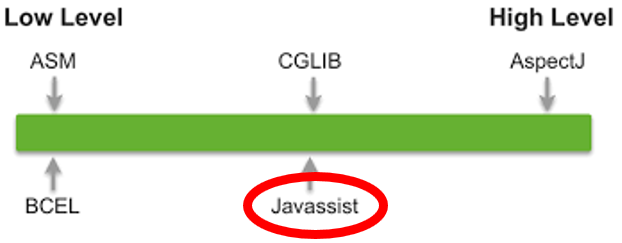
\includegraphics[width=0.8\linewidth]{bytecodeModificationLevels}
\caption{Bytecode modification levels}
  \label{fig:bytecodeModificationLevels}
\end{figure}

Unlike many other libraries Javassist offers two levels of API: source level and bytecode level (See figure \ref{fig:bytecodeModificationLevels}). Using the source-level API, the user can edit a class file without any familiarity with the specifications of the Java bytecode. Only knowing the Java language is enough because the API is designed only with the vocabulary of Java. On this level the programmer just has to write normal source code and Javassist compiles it automatically. The bytecode level allows the user to modify classes directly in binary form like other editors, e.g. ASM.

At this point, let us look at a small example to give you an idea how the bytecode manipulation works.

\begin{figure}[H]
\centering
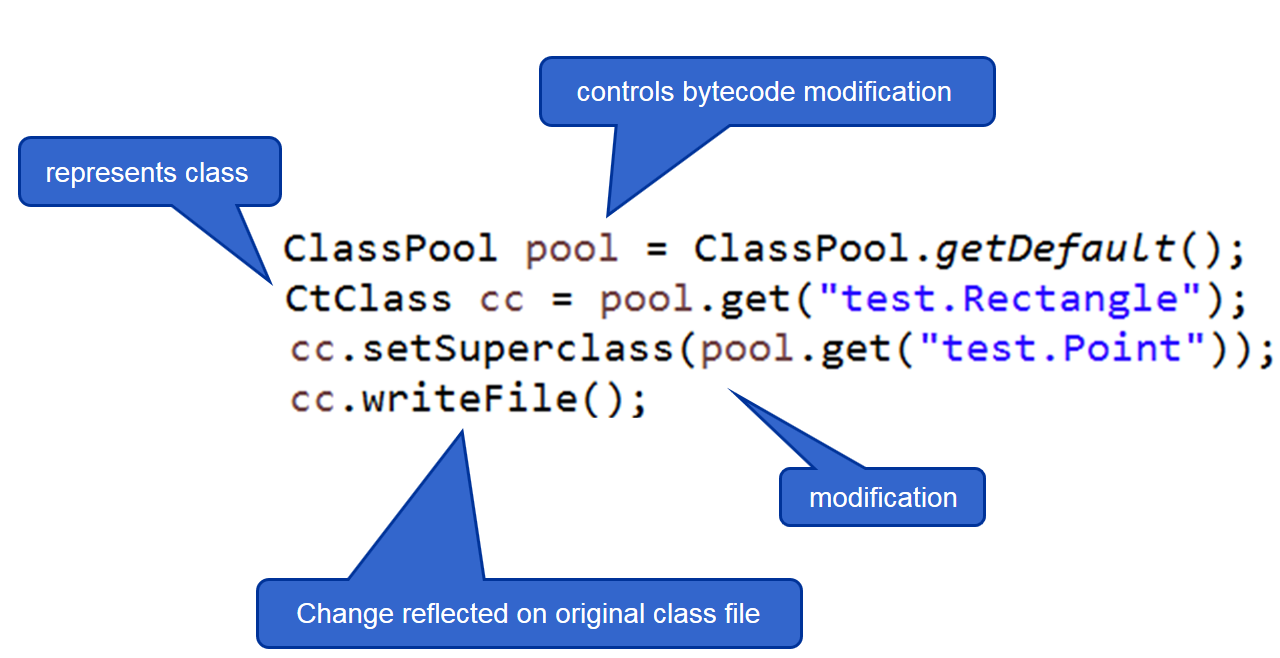
\includegraphics[width=0.8\linewidth]{javassistExample}
\caption{Javassist example}
  \label{fig:javassistExample}
\end{figure}

First a ClassPool object is obtained that controls bytecode modification with Javassist. With the ClassPool a class file can be read on demand for constructing a CtClass object. The class CtClass (compile-time class) is just an abstract representation of a class file which means all manipulations are performed on the CtClass. With the method invocation \textit{get()} on ClassPoola reference to the class file \textit{test.Rectangle} is obtained. In this example the superclass of \textit{test.Rectangle} is just changed to \textit{test.Point}. If the changes are done, the method call \textit{writeFile()} on CtClass is necessary to make sure that the changes are reflected on the original class file.\footnote{Getting started with Javassist: \url{http://jboss-javassist.github.io/javassist/tutorial/tutorial.html}}

\begin{figure}[H]
\centering
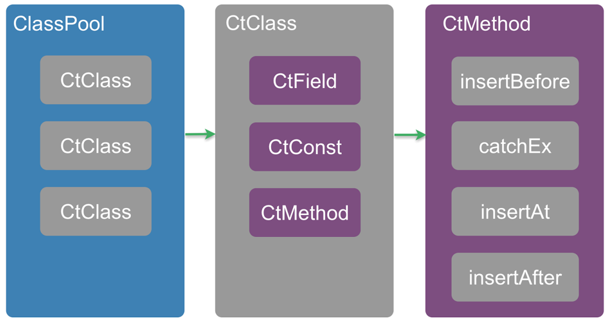
\includegraphics[width=0.8\linewidth]{javassistModules}
\caption{Javassist Modules}
  \label{fig:javassistModules}
\end{figure}

Figure \ref{fig:javassistModules} gives you an understanding/overview how the main part of bytecode manipulation with Javassist is built up. The ClassPool is nothing else than a container of multiple CtClasses. As described before CtClass is just the abstract representation of a class file on which modifications are done. Like typical classes, it can hold several compile-time fields, constants or methods. While speaking about bytecode manipulation all the time, nothing but editing methods is manly meant. It is possible to insert additional source code at the beginning of the method body, at the end or at a specific line. Next to these options even a \textit{catchBlock} can be added.

\begin{figure}[H]
\centering
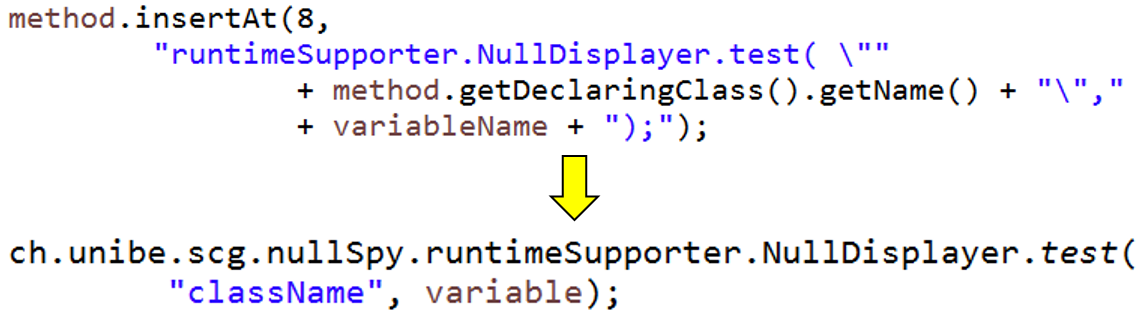
\includegraphics[width=0.9\linewidth]{insertionCodeExample}
\caption{Inserting code example}
  \label{fig:insertionCodeExample}
\end{figure}

\section{JAD}
JAva Decompiler\footnote{\url{https://sourceforge.net/projects/jadclipse/}} is a decompiler and a Eclipse plugin for the programming language Java. A short explanation what a decompiler is: a computer program that takes an executable file as input, and attempts to create a high level, compatible source file that does the same thing. So it is used in software reverse engineering.

\begin{figure}[H]
\centering
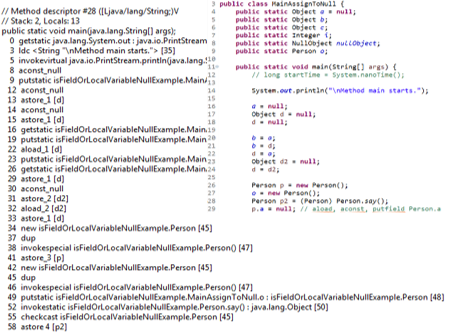
\includegraphics[width=0.6\linewidth]{bytecodeSourcecode}
\caption{Decompile example}
  \label{fig:bytecodeSourcecode}
\end{figure}

JAD is used in NullSpy since after running NullSpy on a project only the modificated bytecodes are available. To simplify the check whether the modification by Javassist, e.g. inserting source code, has succeeded, a decompiler is needed.

\chapter{NullSpy}
As earlier explained in the introduction (\ref{ch:introduction}), this project is about providing the user with additional stack trace where the origin of a NullPointerException is actually rooted. Briefly worded, it shows the developer the exact location of where a method receiver, which causes the NPE, was assigned to null.

This is the main chapter of the thesis. Here we would like to give you a short insight of how we managed to successfully implement the core of the project NullSpy. Next to how it is built up, we will also let you know what challenges we were encountering during the implementation and about the limitations we planned for future work (\ref{ch:conclusionsFutureWork}).


\section{High level overview/Rough Scheme}
\label{sec:highLevelOverview}
The general approach of NullSpy is to statically analyze and add additional bytecode to a project. After reading the section Javassist (\ref{sec:javassist}) you should be more familiar with how bytecode manipulation with Javassist works.

What NullSpy first does is loading the project you want it to be able to track the null assignment if a NullPointerException is thrown. By loading the project to NullSpy, the compiled class files of the project are addressed only, which means the project itself does not have to be imported to the programming environment, e.g. Eclipse. Simultaneously at load time each class file is modified with help of Javassist; In what way will be discussed in the following section “Low level overview”.

Once the project modification is done it is stored in a destination folder that the user has chosen before. This means after the changes there will be another version of the project which can do additional stuff like tracking the null assignment. Because only the class files are accessed previously, the result which is stored in the destination folder is as expected only the modified bytecode.

The reason why we store the modified project in another directory than overwriting the existing one is because we would like to only involve Javassist library in the loading and editing part. This means the execution of the altered project does not include Javassist. This way the user does not have to download Javassist and integrate it to the project.

How do we check whether the instrumentation worked and the project really tracks the null assignment? The answer is wrapping the modified project into a jar file with which the modified project can be executed in the terminal or in Eclipse.

\begin{figure}[H]
\centering
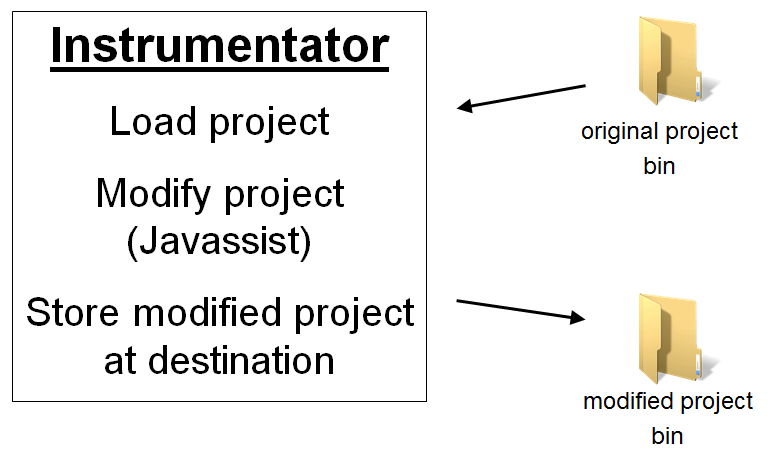
\includegraphics[width=0.5\linewidth]{highLevelOverview}
\caption{Modification overview}
  \label{fig:highLevelOverview}
\end{figure}


\section{Low level overview}
NullSpy only handles the unhandled NullPointerException, meaning the main method of a project is wrapped with a \textit{''catchBlock''} where the NPE is treated. The idea in this \textit{''catchBlock''} is to load the data about the assignments and about the method receiver to compare them with each other. With the stacktrace the line number and the name of the Java class of where the NPE occured can be figured out. We look them up in the method receiver information and get some hold points with which we look up in the assignment information. If there is a match we provide the user with an additional stacktrace next to the usual one. Thanks to that link that points directly to the NPE root, debugging will be easier or it can even be skipped or avoided completely. To be able to provide this function data about the method receiver and variable assignment have to be collected initially. 

So we first load the project which should be modified and then go through all class files of it. A NullPointerException can only be thrown if a method call was performed on a method receiver which is null. That means we have to gather information about the method receiver. Next to this also information about the variable assignments has to be collected to know the exact location of the null assignment. The main idea behind NullSpy actually is to get information comparing those together when a NullPointerException occurs and if there is a hit during the comparison the  location of the null assignment can be obtained easily.

The implementation behind the NullSpy concept will be explained more fully.

\subsection{Method Receiver Data Collection}
\label{subsec:methodReceiver}
Unfortunately, Javassist does not provide the function to directly get the method receiver. We got a suggestion to use AST (Abstract Syntax Tree footnote wiki) to get it but we decided to not go deeper into this and implement our own algorithm.

The algorithm contains following steps (abstract):\newline\newline
\fbox{
\label{alg:methodReceiverAlg}
\begin{minipage}{\linewidth}
\begin{enumerate}
\itemsep8pt
      \item Getting pc-interval of method invocation
      \item Storing all possible method receiver interval within the interval of step 1 into an ArrayList
			\item Getting the number of parameters, the method invocation takes
			\item Traversing back the ArrayList the amount of parameters obtained in step 3
			\item Result: method receiver interval
			\item Store variable name, type etc. into an external csv file
   \end{enumerate}
	\end{minipage}
	}
\newline\newline\newline
In step 1 we had big troubles getting the right interval of the method receiver because only by statically analyzing the bytecode it is unapparent where the method receiver is situated exactly. But more about the challenges you will learn more in chapter \ref{subsec:methodReceiverDifficulties}.

Statically analyzing bytecode for method receiver means looking for certain opcodes which matches all opcodes that matches with the regex \textit{''invoke.*''}}. There are exactly five kinds of bytecode instruction: \textit{invokedynamic}, \textit{invokeinterface}, \textit{invokespecial}, \textit{invokestatic}, \textit{invokevirtual}. The invocation opcode invokedynamic facilitates the dynamic-typed languages\footnote{Language whose type checking is usually performed at runtime.} through dynamic method invocation. In our case it can be ignored because NullSpy only supports the static-typed language\footnote{Language whose type checking is performed at compile time.} Java.

In case of the \textit{invokestatic} instruction we do not have a method receiver. That is why NullSpy treats it extraordinary like ignoring it completely or wrap it as a possible method receiver when it is actually a parameter of a method invocation. In all other cases we normally use the algorithm to get the method receiver. The gathered data about method receivers are stored in an external \textit{csv} file due to performance and overhead minimization.

\subsection{Variable Data Collection}
\label{subsec:variable}
While going through the bytecode attention is paid to some opcodes\footnote{Operation code: Machine language instruction.}. Right after each keyword that indicates a variable assignment we insert some bytecode. The inserted code represents a test method which tests whether the value of the assigned variable is null or not and store some information about it. Unlike in getting information about the method receiver in subsetion \ref{subsec:methodReceiver} the data about the variables are stored in a HashMap.

What kind of opcodes were NullSpy looking for? For instance or class/static variables the bytecode instruction \textit{getfield} and \textit{getstatic} were essential, for local variables the important opcodes were those which matches the regex \textit{''aload.*''}. Due to different types of variables and the limitation of Javassist gathering information about them was performed differently. Again getting the necessary data about the variables we encountered many difficulties which will be discussed in the subsection \ref{sec:challenges}.

\subsubsection{Local Variable}
\label{subsubsec:localVariable}
Unfortunately, Javassist does not provide any support for gaining information about local variables that is why getting the needed data we had to understand how bytecode is constructed. At this point we would like to give you a small bytecode introduction.

\begin{figure}[H]
\centering
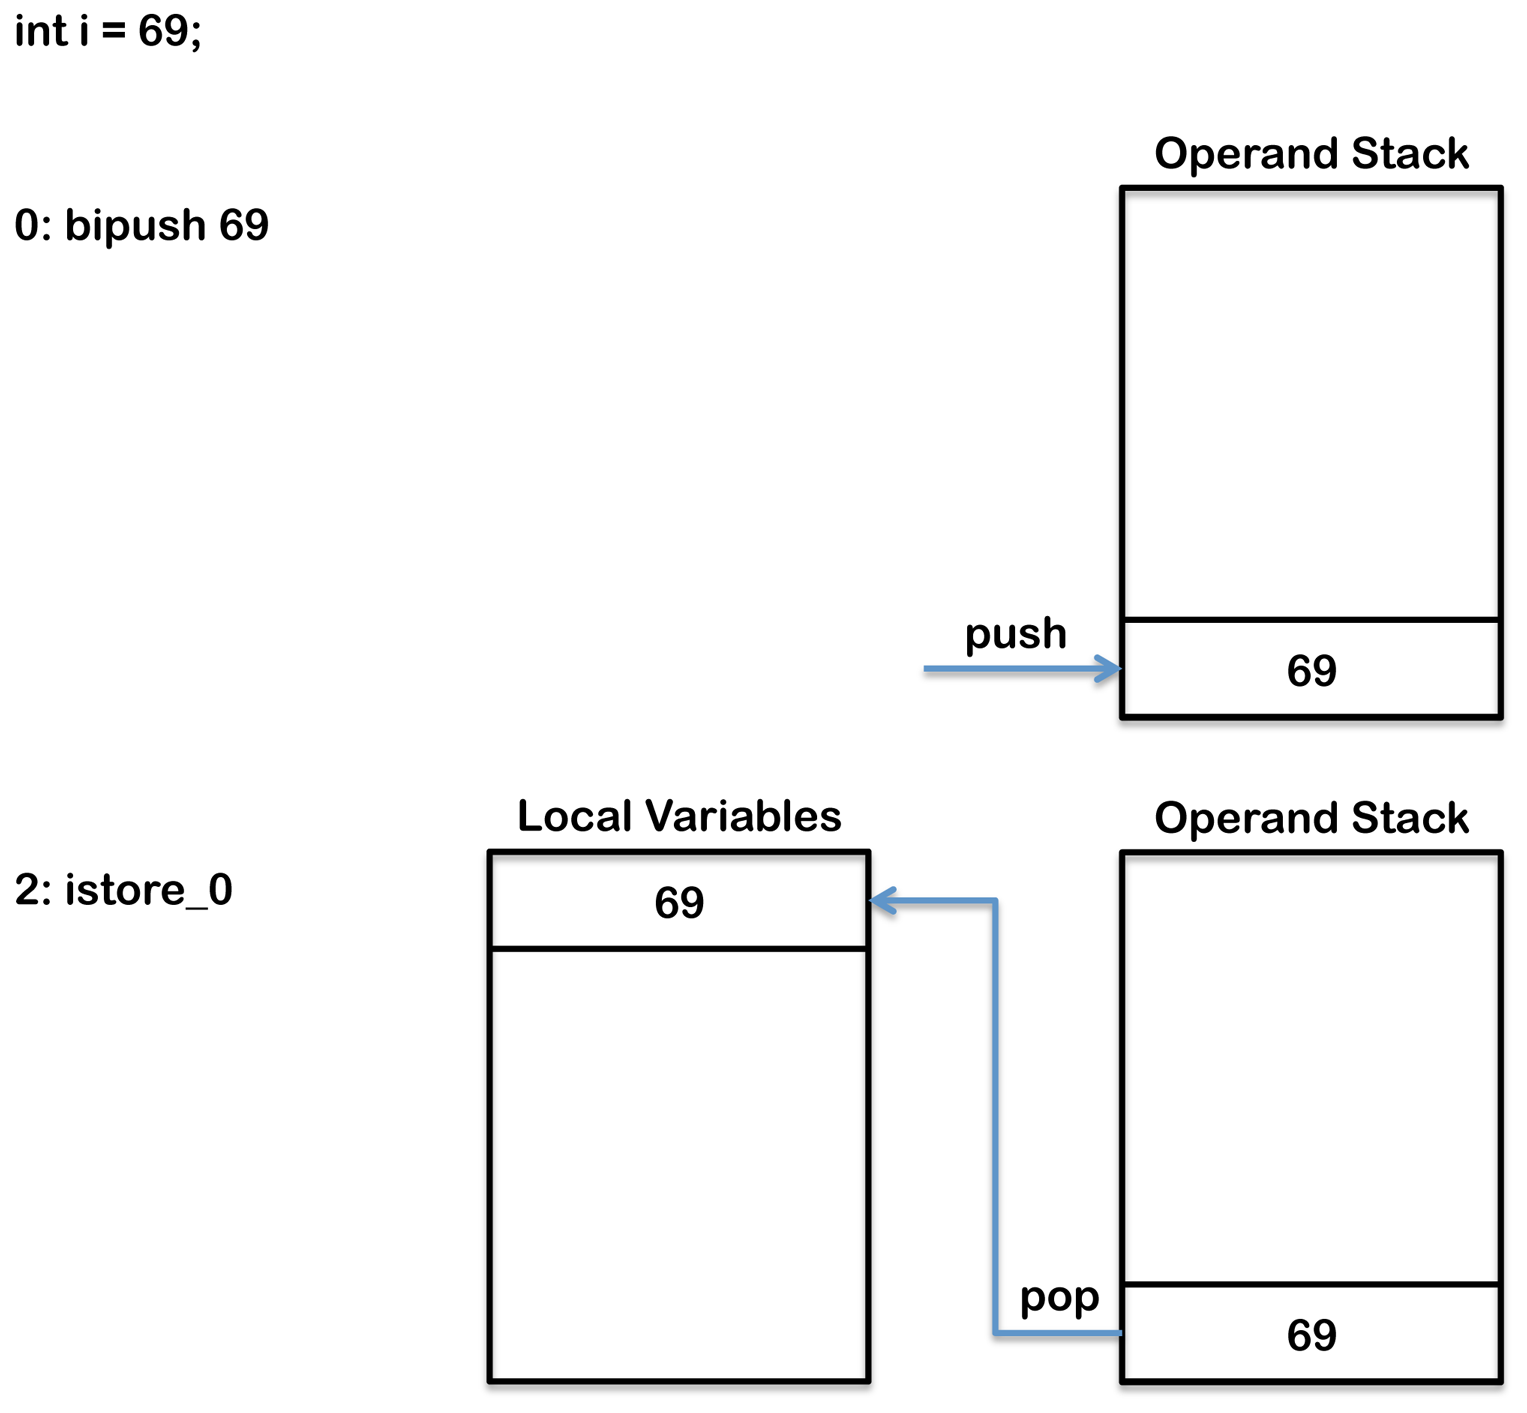
\includegraphics[width=0.5\linewidth]{localVarCreationBytecode}
\caption{Local variable creation bytecode\footnote{\url{http://blog.jamesdbloom.com/images_2013_11_17_17_56/java_local_variable_creation_byte_code.png}}}
  \label{fig:localVarCreationBytecode}
\end{figure}

If a local variable is created, the value assigned to it is pushed onto the operand stack. With the bytecode instruction \textit{''.*store.*''} the local variable is popped from the operand stack and stored into a local variable array slot. In which slot it is stored can be extracted from the instruction. Opcodes for storing local variables is composed of one, or in some cases two bytes. There are reserved machine commands for the first four local variables, index-linked from 0 to 3 and each of them contains one byte (astore\_0, astore\_1, astore\_2, astore\_3). If there is no slot number visible in the instruction, it indicates that the slot number is stored in the second byte from where it can be extracted. Next to storing the local variable loading it from the local variable array is possible to, but only with the local variable slot number.

With this short introduction understanding the local variable table should be easier. Each method of a class file contains a local variable table (see figure \ref{fig:localVarTable}) with which many information can be read out of it, e.g. the lifespan of the local variable, what it is called, in which slot it is stored and what type it has.

\begin{figure}[H]
\centering
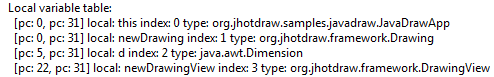
\includegraphics[width=\linewidth]{localVarTable}
\caption{Local variable table}
  \label{fig:localVarTable}
\end{figure}

We had to pay attention to be sure to get the right local variable. Every time when we bumped into the opcode \textit{''.*store.*''} we could only get its slot and the pc\footnote{Program counter/instruction pointer: A processor register that indicates where a computer is in its program sequence.} where it is situated in the bytecode sequence. In the earlier paragraph the lifespan of the local variable was mentioned, the importance behind this is as soon as the lifespan of one ends, the slot can be reused by the next instantiated local variable. This way, the local variable table could contain multiple entries with the same local variable slot.

\begin{figure}[H]
\centering
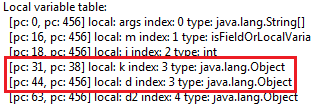
\includegraphics[width=0.7\linewidth]{localVarTableDuplicatedSlot}
\caption{Local variable table entries with same slot}
  \label{fig:localVarTableDuplicatedSlot}
\end{figure}

After extracting the slot of the local variable we will get the first local variable table entry which contains that slot. If the pc of the local variable assignment is not included in the lifespan-pc-interval of the entry, the next entry with the same slot will be checked until both criteria (slot and pc) fits. Once those criteria are met we can be positive about having got the right local variable table entry to extract the information needed.

Next to the local variable table each methods of a class file also holds another attribute called line number attribute. This is just the mapping table from pc to source code line number. Since encountering the storing keyword the pc is available , with help of it the line number can be easily obtained.

\begin{figure}[H]
\centering
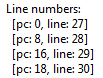
\includegraphics[width=0.3\linewidth]{lineNrTable}
\caption{Line number table}
  \label{fig:lineNrTable}
\end{figure}

\subsubsection{Instance and Class/Static variables (Fields)}
\label{subsec:fields}
Although Javassist does not support the access to local variable it provides a way for fields. Javassist allows modifying an expression in a method body with the class \textit{Javassist.expt.ExprEditor}. In our case we only want to extract some information about the fields instead of any modification, nevertheless this class can be used appropriately. What it does is to scan the bytecodes on instructions like \textit{''putfield''} or \textit{''putstatic''}.

There are only two instructions that indicates an access to a field, but there are actually many different types. To get the meaning of different types see the following list:\newline\newline
\fbox{
\begin{minipage}{\linewidth}
(\textbar\dots\textbar: put value on operand stack for assigning to a field)
\begin{enumerate}
\itemsep8pt
      \item aload\_0, \textbar\dots\textbar, putfield
      \item \textbar\dots\textbar, putstatic
			\item aload.*, \textbar\dots\textbar, putfield
			\item aload\_0, (getfield)+, \textbar\dots\textbar, putfield
			\item getstatic, (getfield)*, \textbar\dots\textbar, putfield
   \end{enumerate}
	\end{minipage}
	}
	
Depending on the category the field belongs, different kind of information is stored. For fields 1-2 following information is needed and stored:\newline\newline
\fbox{
\begin{minipage}{\linewidth}
\begin{itemize}
\itemsep8pt
      \item fieldID (which is field or localVar)
\item fieldname
\item fieldType
\item fieldDeclaringClassName (in which class it is instantiated)
\item isFieldStatic
\item fieldLineNumber
\item startPosition (nonstatic: this; static: value loading bytecode for assigning to the field)
\item storePosistion (putfield/putstatic)
\item afterStorePosition (right before this pos additional bytecode is inserted)
\item classWhereFieldIsAccessed (in this case the same as fieldDeclaringClassName)
\item behavior (method where it is accessed)
\item indirectVariable (null - explained immediately)
   \end{itemize}
	\end{minipage}
	}
\newline

In NullSpy we call these fields \textit{''directFields''}. After reading \textit{''direct''} you surely think of there must be something like \textit{''indirectFields''}, and that is right. As \textit{''indirectFields''} the fields 3-4 are numbered among. Everything before the instruction \textit{putfield} is termed as \textit{''indirectVariable''}. For those fields more data are needed to store for their identification. Nearly the same as above, except: \newline\newline
\fbox{
\begin{minipage}{\linewidth}
\begin{itemize}
\itemsep8pt
      \item classWhereFieldIsAccessed (can be differend than fieldDeclaringClassName)
\item indirectVariable:
\begin{itemize}
\item indirectVariableName
\item indirectVariableType
\item indirectVariableDeclaringClassName
\item isIndirectVariableStatic
\item indirectVariableOpcode (to distinguisch if it is a localVariable or a field)
\end{itemize}
   \end{itemize}
	\end{minipage}
	}
\newpage
\lstinputlisting[language=java]{code/Fields.java}

Once included more bytecode, getting the data of fields needed some adaptation (see \ref{subsec:variableDifficulties}).

\subsection{Bytecode Adaptation}
\label{bytecodeAdaptation}
Each time encountering a variable assignment we first extract the needed data and directly after this we adapt the class file by adding extra bytecode right after the assignment bytecode to check whether the variable is null or not. If it is null, the information collected before is stored either into the \textit{''localVariableMap''} or into a \textit{''fieldMap''} which are HashMaps.

The added bytecode represents a static method of a class named \textit{ch.scg.nullSpy.runtimeSupporter.VariableTester} which will be added to the modified project after class file modification is done. Depending on the kind of variable analyzed at the moment different bytecode is constructed, meaning different method with different parameter/variable data is added.

There were again some challenges we had to get over, like getting the wanted data after an instrumentation and entering the additional code in the right position of the bytecode sequence (\ref{subsec:bytecodeAdaptationDifficulties}).

Once we have gone through the bytecode of a Java class, the modified class files are stored in a destination directory as mentioned in \ref{sec:highLevelOverview}. Next to the instrumentation supplementary supporter classes are added to the project. The most important ones are \textit{ch.unibe.scg.nullSpy.runtimeSupporter.VariableTester} which tests whether a variable is null or not and \textit{ch.unibe.scg.nullSpy.runtimeSupporter.NullDisplayer} which matches data and prints the location of a null assignment when a NullPointerException is thrown.


\section{Challenges}
\label{sec:challenges}
In this section we could like to give you an understanding of few difficulties occurred during the implementation of NullSpy.

\subsection{Obtaining Method Receiver Data Difficulties}
\label{subsec:methodReceiverDifficulties}
Aforementioned in subsection \textit{Method Receiver Data Collection} \ref{subsec:methodReceiver} we were encountered with a persistent problem, namely getting the pc-interval of the method receiver when the interval covers multiple lines in source code. In many development environment the written code can be formatted automatically and as well manually. See following figures:

\begin{figure}[H]
\centering
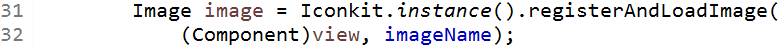
\includegraphics[width=\linewidth]{multipleLine/pic4-1}
\caption{Method invocation split in two lines example}
  \label{fig:pic4-1}
\end{figure}

\begin{figure}[H]
\centering
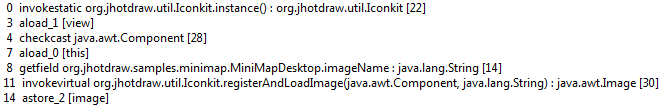
\includegraphics[width=\linewidth]{multipleLine/pic4-2}
\caption{Bytecode to figure \ref{fig:pic4-1}}
  \label{fig:pic4-2}
\end{figure}

\begin{figure}[H]
\centering
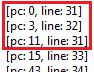
\includegraphics[width=0.3\linewidth]{multipleLine/pic4-3}
\caption{Line number table/interval to figure \ref{fig:pic4-1}}
  \label{fig:pic4-3}
\end{figure}

Figure shows a normal method invocation which is split into two lines in source code. This cannot be figured out by just looking at the bytecode therefore the line number attribute (\ref{fig:lineNrTable}) has to be consulted too. There is no method receiver in the figure because the method receiver would contain a method invocation itself (\textit{''Iconkit.instance()''}, what is not supported in NullSpy. Another method receivers NullSpy does not support are elements of collections due to complex structures that can be stored in the collections. But still it is a good example to show you how the bytecode and the line number attribute for this looks like. Applying the algorithm (\ref{alg:methodReceiverAlg}) for gathering data about method receivers in this situation looks as follows:

\newline\newline
\fbox{
	\begin{minipage}{\linewidth}
		\begin{enumerate}
			\itemsep8pt
			\item pc-interval: \newline 0-11 (cut everything off what has nothing to do with the method invocation)
			\item ArrayList: \newline [0,[3,4],[7,8]]
			\item Number of parameters: \newline 2
			\item Traversing back the amount of parameters: \newline [7,8] (1) \rightarrow [3,4] (2)
			\item Result: \newline 0 (invokestatic) = possible method receiver
			\item Not storing it because NullSpy does not support this kind of method receiver
		\end{enumerate}
	\end{minipage}
}

So how did we get the pc-interval? Just looking at bytecode is not enough, so we are looking at the line number attribute. Line number \textit{31} (\ref{fig:pic4-3}) is listed twice, this indicates that the method invocation is split into multiple line in source code. The former declares the starting point of the interval and the latter the end of it. How to get the pc-interval will be presented shortly. But first take a look at more examples:

\begin{figure}[H]
\centering
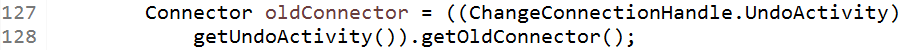
\includegraphics[width=\linewidth]{multipleLine/pic3-1}
\caption{Alternating line number example}
  \label{fig:pic3-1}
\end{figure}

\begin{figure}[H]
\centering
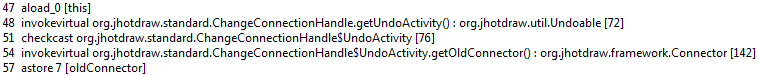
\includegraphics[width=\linewidth]{multipleLine/pic3-2}
\caption{Bytecode to figure \ref{fig:pic3-1}}
  \label{fig:pic3-2}
\end{figure}

\begin{figure}[H]
\centering
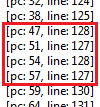
\includegraphics[width=0.3\linewidth]{multipleLine/pic3-3}
\caption{Line number table/interval to figure \ref{fig:pic3-1}}
  \label{fig:pic3-3}
\end{figure}

Special about this example is that the multiple line interval does not start with the smaller line number and end with the bigger one, apart from that it is alternated stored in the line number attribute.

\begin{figure}[H]
\centering
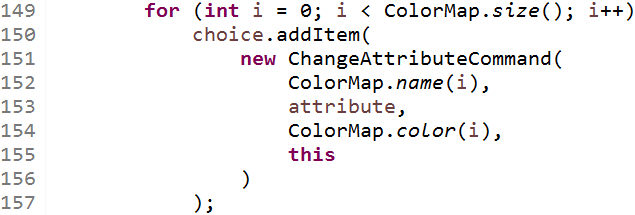
\includegraphics[width=\linewidth]{multipleLine/pic2-1}
\caption{Nested interval example}
  \label{fig:pic2-1}
\end{figure}

\begin{figure}[H]
\centering
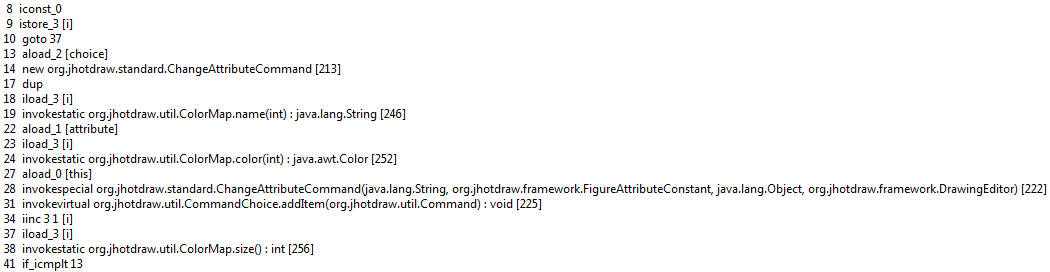
\includegraphics[width=\linewidth]{multipleLine/pic2-2}
\caption{Bytecode to figure \ref{fig:pic2-1}}
  \label{fig:pic2-2}
\end{figure}

\begin{figure}[H]
\centering
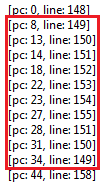
\includegraphics[width=0.3\linewidth]{multipleLine/pic2-3}
\caption{Line number table/interval to figure \ref{fig:pic2-1}}
  \label{fig:pic2-3}
\end{figure}

Neither in bytecode nor in line number attribute we can extract the exact interval of method invocations. Generally, we cannot distinguish if the interval represents a method invocation or a loop. Another interesting thing is that in the figure multiple corresponding pcs are included.

\begin{figure}[H]
\centering
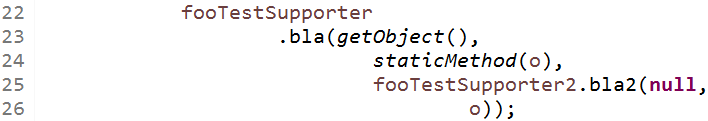
\includegraphics[width=\linewidth]{multipleLine/pic5-1}
\caption{Uncomplete interval example}
  \label{fig:pic5-1}
\end{figure}

\begin{figure}[H]
\centering
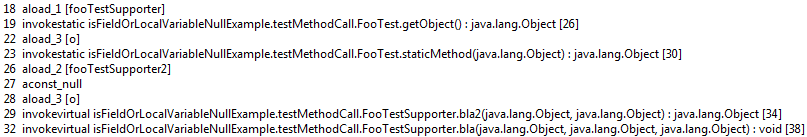
\includegraphics[width=\linewidth]{multipleLine/pic5-2}
\caption{Bytecode to figure \ref{fig:pic5-1}}
  \label{fig:pic5-2}
\end{figure}

\begin{figure}[H]
\centering
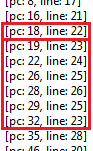
\includegraphics[width=0.3\linewidth]{multipleLine/pic5-3}
\caption{Line number table/interval to figure \ref{fig:pic5-1}}
  \label{fig:pic5-3}
\end{figure}

By using the algorithm we only get the interval from pc 19-32, but actually pc 18 also belongs to the interval. That the missing pc is missing will be detected in step 4\&5 when traversing back the ArrayList by the number of parameters. If it is not a static method invocation and there is not enough possible method receivers stored in that ArrayList to traverse back, the missing pc is added in retrospect.

	\lstinputlisting[language=java]{code/MultipleLinePseudoCode.java}

This pseudocode will give you the main or a very rough idea how the invocation interval can be gained. If you are interested in knowing the exact way, please see the implementation of the class \textit{ch.unibe.scg.nullSpy.instrumentator.controller.methodInvocation.MultipleLineManager} and \textit{ch.unibe.scg.nullSpy.instrumentator.controller.methodInvocation.MethodInvocationAnalyzer}.

\subsection{Obtaining Variable Data Difficulties - Fields}
\label{subsec:variableDifficulties}
We previously mentioned that NullSpy first collects data about fields and we met some difficulties regarding this. By using the method \textit{loopBody()} from class \textit{Javassist.expt.ExprEditor} (\ref{subsec:fields}) for gathering information caused those troubles because it loops through the GIVEN \textit{methodInfo} which contains the bytecode sequence of a method. Even after finding a field assignment and adding some additional bytecode to it, the method still iterates through the unchanged \textit{methodInfo} it got as parameter without the additional bytecode. Getting the right startPc of a field assignment is not a straight forward process as it may seem.

After entered extra instructions the method \textit{loopBody} iterates onwards until it finds a key which indicates an access to a field. Normally, Javassist provides a method with which the starting pc of the field access can be find out easily, but in our case not due to bytecode alternation. This method returns the starting pc of the field as if there was no changes, however it actually has to return a bigger starting pc than it does. The starting pc is needed to distinguish in what category the field has to be assigned to (\ref{subsec:fields}).

To find the right starting pc of the field assignment we compare the starting pc which a method of Javassist returns with the \textit{afterStorePc} of the previously found field assignment. Every time an assignment is found we store it as a reference for obtaining right data. Even for the storing pc of an assignment (\textit{''put.* ''} the last found field is essential. If there is more interest how those pcs are obtained, please see the class \textit{ch.unibe.scg.nullSpy.instrumentator.controller.FieldAnalyzer}.

\subsection{Bytecode Adaptation Difficulties}
\label{subsec:bytecodeAdaptationDifficulties}
The reason why we decided to use Javassist for our NullSpy project is because the thought of only using the source-level API \ref{fig:bytecodeModificationLevels} to implement everything. It would have been much easier to only operate at source-level instead of learning how to read bytecode or extract data from it or enter extra code into it, yet at the end we still had to do everything at bytecode-level.

One big problem encountered while inserting the test method between an assignment and a closing bracket \textit{''\}''}. We tried to insert additional code as shown in figure \ref{fig:insertionCodeExample} by specifying the exact line number where it should be entered in source code. Unfortunately Javassist first checks the specified line whether it contains some code (only symbols excluded). If there is no code at that line it computes the next line that contains some and inserts the test method right before it. Please visualize a situation where for example a local variable is created/instantiated at the end of a \textit{if-body}. In this situation Javassist adds the extra code right before the next code line which is outside the existing scope of the local variable.

\begin{figure}[H]
\centering
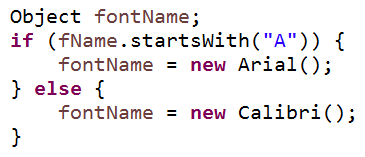
\includegraphics[width=0.7\linewidth]{bytecodeAdaptionExample_1}
\caption{Bytecode adaptation example}
  \label{bytecodeAdaptationExample_1}
\end{figure}

\begin{figure}[H]
\centering
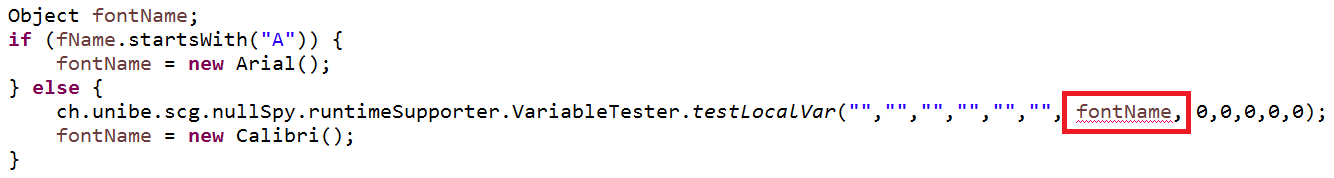
\includegraphics[width=0.7\linewidth]{bytecodeAdaptionExample_2}
\caption{Wrong Adaptation to \ref{bytecodeAdaptationExample_1}}
  \label{bytecodeAdaptionExample_2}
\end{figure}

That is why changed the way to insert the test method at bytecode-level. Like this we first have to build up the bytecode sequence and then enter it before a specific pc. Please take a look at the class \textit{ch.unibe.scg.nullSpy.instrumentator.controller.ByteCodeAdapter} how the bytecode sequence is created.

There are of course many other small problems during the implementation of NullSpy but these mentioned are the most troublesome ones.

\section{Limitations}
...

\chapter{Validation}
In which you show how well the solution works.

\section{JHotDraw}
JHotDraw
To check whether the logic of the bytecode manipulation in this project NullSpy is working as desired, we had to perform them on a large working project. Thanks to Nevena Milojkovi\'{c} and her experience with the combination Javassist and JHotDraw we as well decided to test NullSpy on the project JHotDraw.
It is an open-source Java GUI framework for technical and structured Graphics. Its original authors have been Erich Gamma and Thomas Eggenschwiler. 

\chapter {Conclusion and Future Work}
\label{ch:conclusionsFutureWork}
In which we step back, have a critical look at the entire work, then conclude, and learn what lays beyond this thesis.

\chapter {Anleitung zu wissenschaftlichen Arbeiten}
This consists of additional documentation, e.g. a tutorial, user guide etc.
Required by the Informatik regulation.

%END Doc
%-------------------------------------------------------

\bibliography{thesis}
\bibliographystyle{plain}

\clearpage
\thispagestyle{empty}
\null\vfill
\begin{center}
''Ich erkl\"are hiermit, dass ich diese Arbeit selbstst\"andig verfasst und  keine  anderen  als  die  angegebenen  Quellen  benutzt  habe. 
Alle Stellen, die w\"ortlich oder sinngem\"ass aus Quellen entnommen  wurden,  habe  ich  als  solche  gekennzeichnet.  Mir  ist  bekannt,  dass  andernfalls  der  Senat  gem\"ass  Artikel 36  Absatz 1 Buchstabe 
r  des  Gesetzes  vom  5. September 1996  \"uber  die  Universit\"at zum Entzug des auf  Grund dieser Arbeit verliehenen Titels berechtigt ist.“
\vfill
\clearpage

\end{document}